\section*{Work for This Year}

\begin{frame}{Laptime Simulation}
    \begin{figure}
        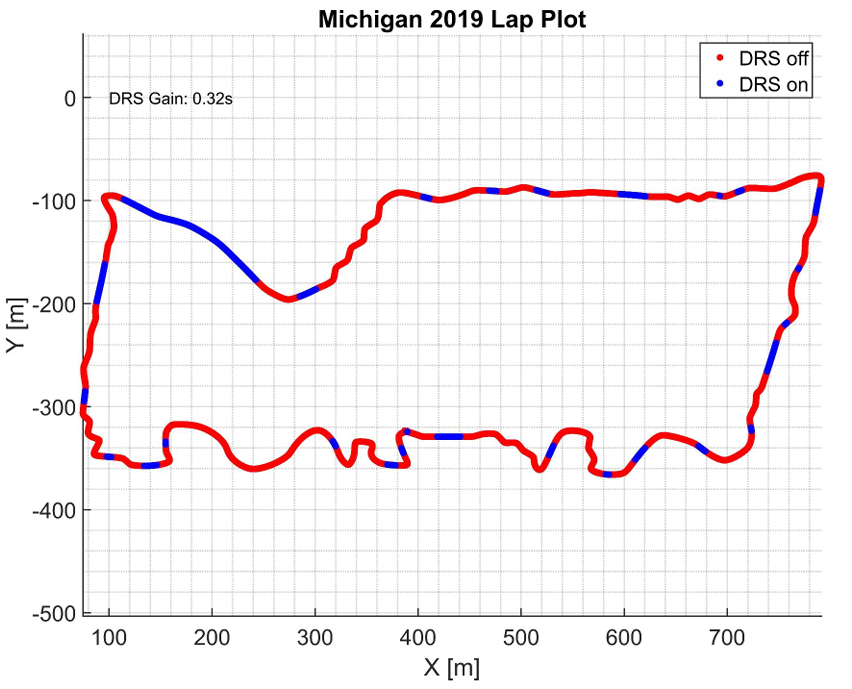
\includegraphics[width=0.5\textwidth]{res/DRS Simulation.png}
    \end{figure}
    Laptime simulation can answer questions like:
    is it worth it to use DRS\@?
    What is the optimal final drive ratio?
    Should aero focus on increasing lift or decreasing drag?
    \textbf{Questions about the track}.
\end{frame}

\begin{frame}{Lapsims}
    Existing Simulations:
    \begin{itemize}
        \item \textbf{OpenLAP:} Open-source point mass laptime simulation
        \item \textbf{Bailey's Lapsim:} Custom lapsim with better tyre model
        \item \textbf{Murray's Lapsim:} Four corner lapsim  with better features
    \end{itemize}
    Problems:
    \begin{itemize}
        \item Doesn't model electric powertrain accurately
        \item Not accessible for wider team to use (complex to install)
        \item Code is difficult to maintain or add new features
    \end{itemize}
    \begin{block}{The Vision}
        \begin{center}
            \textit{\textbf{Oliver's Lapsim:}
                New lapsim with transient powertrain simulation,
                written in Python, documented}
        \end{center}
    \end{block}
\end{frame}

\begin{frame}{Other Projects}
    \textbf{Driver-in-the-Loop Simulation:}
    Setting up a real-time simulation using IPG software
    so that we can simulate driving the USM car.
    Our drivers could do virtual ``test laps" with different setups.
    \\~\\
    \textbf{Engineering Challenge / Sim Series:}
    A series of scenarios where you act as race engineers and test drivers
    to tune the setup and performance of a car (begins November).
    \\~\\
    \textbf{Testing Planning:}
    Creating a schedule for pre-season testing.
    Deciding what data we would like,
    and how we can measure it.
    Tuning the car (springs/dampers, ride heights, tyre pressure, etc.)
\end{frame}